% 组件库：presentation.tex 之外「以后可能要用」的元素，每个 frame 一个，都编译验证过。
% 用法：需要哪个就把对应 frame（和它用到的宏包）复制进 presentation.tex。
% 只用 TeX Live 常见宏包（tikz、pgfplots、listings、tcolorbox、qrcode、natbib、appendixnumberbeamer、mwe 的示例图）。
\documentclass[aspectratio=169,10pt]{beamer}
\usetheme{Madrid}
\usecolortheme{default}

\usepackage{booktabs}
\usepackage{colortbl}       % 表格行着色（\rowcolor）
\usepackage{multirow}
\usepackage{array}
\usepackage{graphicx}
\usepackage{amssymb}
\usepackage{mathtools}
\usepackage{subcaption}
\usepackage{tikz}
\usetikzlibrary{arrows.meta, positioning, shapes.geometric}
\usepackage{pgfplots}
\pgfplotsset{compat=1.16}
\usepackage{listings}
\usepackage{tcolorbox}
\usepackage{qrcode}
\usepackage[round]{natbib}
\usepackage{appendixnumberbeamer}   % 附录页不计入总页数

\lstset{basicstyle=\ttfamily\scriptsize, keywordstyle=\color{blue!70!black}\bfseries,
        commentstyle=\color{green!45!black}, stringstyle=\color{red!60!black},
        frame=single, rulecolor=\color{gray!40}, columns=fullflexible, showstringspaces=false}
\newtcolorbox{keybox}[1][]{colback=blue!4, colframe=blue!50!black, fonttitle=\bfseries\small, title=#1}
\setbeamertemplate{note page}[plain]
% \setbeameroption{show notes on second screen=right}   % 讲稿：放映时右屏显示 \note{}（需 pgfpages）
% 讲义版：\documentclass[handout,...]{beamer} 会合并 overlay，每帧只出一页

\logo{\includegraphics[height=0.45cm]{example-image-a}}   % 右下角 logo；换成机构标志
\titlegraphic{\includegraphics[height=1.0cm]{example-image-b}}

% 每个 section 开头自动插一页目录，高亮当前 section（不需要就删掉这段）
\AtBeginSection[]{
  \begin{frame}{Outline}
    \tableofcontents[currentsection, hideothersubsections]
  \end{frame}
}

\title[Components]{Component Gallery}
\subtitle{Reusable Beamer Elements}
\author[A.~Author]{Author Name}
\institute[Univ.]{Institution}
\date{Reference Deck}

\begin{document}

\begin{frame}
  \titlepage
\end{frame}

% ------------------------------------------------------------------
\section{Text and Math}

\begin{frame}{Blocks and Theorems}
  \begin{columns}[T]
    \begin{column}{0.48\textwidth}
      \begin{block}{Block}
        Neutral statement.
      \end{block}
      \begin{alertblock}{Alert block}
        Warning or limitation.
      \end{alertblock}
      \begin{exampleblock}{Example block}
        Example or takeaway.
      \end{exampleblock}
    \end{column}
    \begin{column}{0.48\textwidth}
      \begin{definition}
        A model is \emph{scale-equivariant} if $f(\alpha x) = \alpha f(x)$.
      \end{definition}
      \begin{theorem}
        Built-in environments: theorem, lemma, corollary, definition, example, proof.
      \end{theorem}
      \begin{keybox}[tcolorbox]
        A highlighted box with its own colors.
      \end{keybox}
    \end{column}
  \end{columns}
\end{frame}

\begin{frame}{Overlays: Reveal Step by Step}
  \begin{itemize}[<+->]
    \item Each item appears on the next click
    \item \alert<3>{This one turns red on step 3}
    \item The last item
  \end{itemize}
  \only<4>{\vspace{6pt}Text shown only on step 4 (takes no space before).}
  \uncover<4>{\vspace{6pt}Text uncovered on step 4 (space reserved).}
\end{frame}

\begin{frame}{Equations}
  \begin{equation}
    s_\alpha = \frac{\log \hat y(\alpha P) - \log \hat y(P)}{\log \alpha}
    \label{eq:slope}
  \end{equation}
  \begin{align*}
    \mathcal{L} &= \underbrace{\mathcal{L}_{\text{text}}}_{\text{answer}}
                 + \lambda\, \underbrace{\mathcal{L}_{\text{mask}}}_{\text{segmentation}} \\
                &= \mathcal{L}_{\text{text}} + \lambda \bigl(\mathcal{L}_{\text{bce}} + \mathcal{L}_{\text{dice}}\bigr)
  \end{align*}
  Highlight a term: $y = \colorbox{yellow!40}{$\alpha$}\, x$.
\end{frame}

% ------------------------------------------------------------------
\section{Figures and Tables}

\begin{frame}{Side-by-Side Figures}
  \begin{figure}
    \begin{subfigure}{0.31\textwidth}
      \includegraphics[width=\linewidth]{example-image-a}
      \caption{First}
    \end{subfigure}\hfill
    \begin{subfigure}{0.31\textwidth}
      \includegraphics[width=\linewidth]{example-image-b}
      \caption{Second}
    \end{subfigure}\hfill
    \begin{subfigure}{0.31\textwidth}
      \includegraphics[width=\linewidth]{example-image-c}
      \caption{Third}
    \end{subfigure}
  \end{figure}
\end{frame}

{\setbeamertemplate{navigation symbols}{}
\begin{frame}[plain]
  \begin{tikzpicture}[remember picture, overlay]
    \node at (current page.center) {\includegraphics[width=\paperwidth, height=\paperheight]{example-image}};
    \node[fill=white, opacity=0.85, text opacity=1, inner sep=6pt, anchor=south west]
      at ([shift={(0.4cm,0.4cm)}]current page.south west) {\small Full-bleed image frame with a caption box};
  \end{tikzpicture}
\end{frame}
}

\begin{frame}{Wide Table with Highlighted Row}
  \centering
  \resizebox{\linewidth}{!}{%
  \begin{tabular}{@{}lcccccccc@{}}
    \toprule
    Model & A & B & C & D & E & F & G & H \\
    \midrule
    Baseline 1 & 21.7 & 30.2 & 25.3 & 15.0 & 10.5 & 21.2 & 31.5 & 24.4 \\
    Baseline 2 & 13.3 & 11.6 & 9.8 & 12.0 & 7.5 & 13.9 & 13.0 & 11.9 \\
    \rowcolor{blue!8} Ours & \textbf{31.7} & \textbf{37.2} & \textbf{38.7} & \textbf{37.5} & \textbf{21.1} & \textbf{28.5} & \textbf{48.9} & \textbf{34.8} \\
    \bottomrule
  \end{tabular}}\\[3pt]
  {\scriptsize \texttt{\textbackslash resizebox} fits a wide table to the slide; \texttt{\textbackslash rowcolor} needs \texttt{colortbl}.}
\end{frame}

\begin{frame}{Plot from Inline Data (pgfplots)}
  \centering
  \begin{tikzpicture}
    \begin{axis}[width=0.62\textwidth, height=0.5\textheight, xlabel={scale $\alpha$}, ylabel={$\delta_{1.25}$},
                 xmode=log, log basis x=2, xtick={0.5,1,2}, xticklabels={0.5,1,2},
                 legend pos=outer north east, legend style={font=\scriptsize}, grid=major, grid style={gray!20}]
      \addplot+[mark=*, thick] coordinates {(0.5,29.9) (1,25.9) (2,2.2)};
      \addplot+[mark=square*, thick] coordinates {(0.5,39.8) (1,36.3) (2,25.0)};
      \legend{Baseline, Ours}
    \end{axis}
  \end{tikzpicture}
\end{frame}

\begin{frame}{Pipeline Diagram (TikZ)}
  \centering
  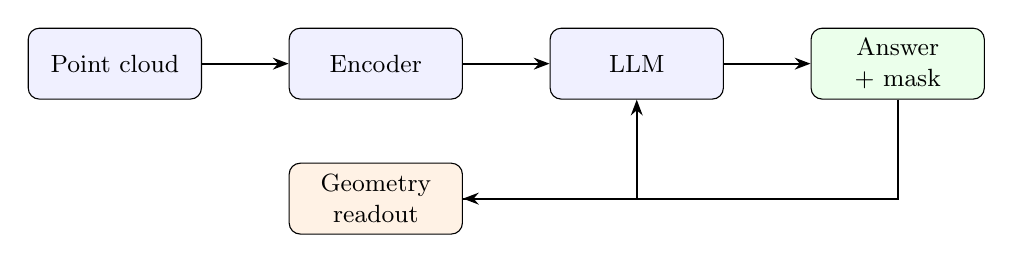
\begin{tikzpicture}[node distance=1.1cm, every node/.style={font=\small},
      box/.style={draw, rounded corners, fill=blue!6, minimum height=0.9cm, minimum width=2.2cm, align=center},
      arr/.style={-{Stealth[length=2mm]}, thick}]
    \node[box] (in) {Point cloud};
    \node[box, right=of in] (enc) {Encoder};
    \node[box, right=of enc] (llm) {LLM};
    \node[box, right=of llm, fill=green!8] (out) {Answer\\+ mask};
    \node[box, below=0.8cm of enc, fill=orange!10] (ro) {Geometry\\readout};
    \draw[arr] (in) -- (enc); \draw[arr] (enc) -- (llm); \draw[arr] (llm) -- (out);
    \draw[arr] (out.south) |- (ro.east); \draw[arr] (ro) -| (llm.south);
  \end{tikzpicture}
\end{frame}

% ------------------------------------------------------------------
\section{Code, Citations, Links}

\begin{frame}[fragile]{Code Listing}
  % 含代码的 frame 必须加 [fragile]
\begin{lstlisting}[language=Python]
def scale_slope(y1, ya, alpha):
    """1 = answer follows the scene, 0 = ignores it."""
    return math.log(ya / y1) / math.log(alpha)   # per question
\end{lstlisting}
  \begin{itemize}
    \item Pseudo-code: use \texttt{lstlisting} without a language, or an \texttt{enumerate}
  \end{itemize}
\end{frame}

\begin{frame}{Citations}
  \begin{itemize}
    \item In text: \citet{chen2020scanrefer} localize objects from language.
    \item In parentheses: grounding benchmarks \citep{chen2020scanrefer, azuma2022scanqa}.
    \item As a footnote\footnote{\citet{azuma2022scanqa}, CVPR 2022.} for slides without a reference page.
  \end{itemize}
  {\scriptsize Compile with \texttt{latexmk} (runs bibtex automatically); references come from \texttt{refs.bib}.}
\end{frame}

\begin{frame}{Paper, Code, and Project Links}
  \begin{columns}[c]
    \begin{column}{0.6\textwidth}
      \begin{itemize}
        \item Paper: \href{https://arxiv.org/}{\texttt{arxiv.org/abs/xxxx.xxxxx}}
        \item Code: \href{https://github.com/}{\texttt{github.com/user/repo}}
      \end{itemize}
    \end{column}
    \begin{column}{0.35\textwidth}
      \centering
      \qrcode[height=2.6cm]{https://github.com/}\\[3pt]
      {\scriptsize scan for the code}
    \end{column}
  \end{columns}
  \note{Speaker note: shown on the second screen when the show-notes option is enabled.}
\end{frame}

% ------------------------------------------------------------------
\section{Closing}

\begin{frame}{References}
  \footnotesize
  \bibliographystyle{plainnat}
  \bibliography{refs}
\end{frame}

{\setbeamertemplate{navigation symbols}{}
\begin{frame}[plain]
  \centering
  \vfill
  {\usebeamerfont{title}\usebeamercolor[fg]{structure}\Huge Thank You}\\[10pt]
  Questions?\\[16pt]
  {\small \texttt{author@institution.edu}}
  \vfill
\end{frame}
}

% 附录：\appendix 之后的页不计入总页数（appendixnumberbeamer），用来放备用页
\appendix
\section*{Backup}
\begin{frame}{Backup: Extra Results}
  Slides for questions; not counted in the page total.
\end{frame}

\end{document}
